\id{ҒТАМР 65.29.03}{}

{\bfseries ЖЕРАЛМҰРТПЕН БАЙЫТЫЛҒАН БИДАЙ КЕБЕГІ МЕН СҰЛЫ ЖАРМАСЫ
НЕГІЗІНДЕГІ ТАҢҒЫ АС ӘЗІРЛЕУ}

\begin{figure}[H]
	\centering
	
\includegraphics[width=0.8\textwidth]{media/pish2/image2}
	\caption*{}
\end{figure}

Н.
\begin{figure}[H]
	\centering
	
\includegraphics[width=0.8\textwidth]{media/pish2/image2}
	\caption*{}
\end{figure}

А.
\begin{figure}[H]
	\centering
	
\includegraphics[width=0.8\textwidth]{media/pish2/image2}
	\caption*{}
\end{figure}

А.
\begin{figure}[H]
	\centering
	
\includegraphics[width=0.8\textwidth]{media/pish2/image2}
	\caption*{}
\end{figure}


\emph{«Қазақ қайта өңдеу және тағам өнеркәсіптері ҒЗИ» ЖШС АФ, Астана,
Қазақстан}

{\bfseries \textsuperscript{\envelope }}Корреспондент-автор:\href{mailto:nurtore0308@gmail.com}{\nolinkurl{nurtore0308@gmail.com}}

Таңғы ас көптеген адамдар үшін танымал таңдау болып табылады, өйткені
олар оңай дайындалады, қоректік және салауатты өмір салтын қолдайды. Бұл
мақалада жералмұртпен байытылған бидай кебегі қосылған сұлы жармасы
негізінде таңғы ас әзірлеу қарастырылды.

Сұлы жармасы талшықтар мен дәрумендердің қажетті мөлшерін қамтамасыз
етеді, ал бидай кебегі минералдардың деңгейін жоғарылатады және ас
қорытуды жақсартады. Инулинге бай жералмұрт тәтті дәм қосады және
ішектің қалыпты микрофлорасын сақтауға көмектеседі. Сонымен қатар, ол
пребиотикалық қасиеттерге ие, бұл асқазан-ішек жолдарының жұмысына
жағымды әсер етеді.

Бұл өнімді әзірлеу сізге күні бойы денсаулық пен энергияны сақтау үшін
қажетті дәрумендер мен микроэлементтермен толықтырылған толық және
теңдестірілген таңғы ас алуға мүмкіндік береді. Экструзия шарттары оның
тағамдық құндылығы мен дәмдік сипаттамаларын сақтай отырып, дайын
өнімнің қытырлақ құрылымын қамтамасыз етеді.

Зерттеу нәтижелері көрсеткендей, әзірленген құрғақ таңғы ас пайдалы ғана
емес, сонымен қатар пайдалы тағамның дәмді нұсқасы болып табылады, бұл
оны тұтынушылардың кең аудиториясы үшін тартымды етеді. Сонымен қатар,
өнімнің жоғары тағамдық құндылығы мен табиғи құрамы қазіргі заманғы
дұрыс тамақтану тенденцияларына сәйкес келеді, бұл оның нарықтағы
сұранысына ықпал етуі мүмкін.

{\bfseries Түйін сөздер:} сұлы жармасы, құрғақ таңғы ас, бидай кебегі,
жарма өнімдері, жералмұрт.

{\bfseries РАЗРАБОТКА СУХОГО ЗАВТРАКА НА ОСНОВЕ ОВСЯНОЙ КРУПЫ С ПШЕНИЧНЫМИ
ОТРУБЯМИ, ОБОГАЩЕННОЙ ТОПИНАМБУРОМ}

{\bfseries М.Султанова, Н.Акжанов\textsuperscript{\envelope }, А.Сәдуакас, А.Камали}

\emph{АФ ТОО «Казахский НИИ перерабатывающей и пищевой промышленности»,
Астана, Казахстан},

e-mail:
\href{mailto:nurtore0308@gmail.com}{\nolinkurl{nurtore0308@gmail.com}}

Сухие завтраки являются популярным выбором для многих людей, так как они
удобны в приготовлении, питательны и способствуют здоровому образу
жизни. В данной статье рассмотрим разработку сухого завтрака на основе
овсяной крупы с добавлением пшеничных отрубей, обогащенного
топинамбуром.

Овсяная крупа обеспечивает необходимое количество клетчатки и витаминов,
в то время как пшеничные отруби повышают уровень минералов и улучшают
пищеварение. Топинамбур, богатый инулином, добавляет сладковатый вкус и
способствует поддержанию нормальной микрофлоры кишечника. Кроме того, он
обладает пребиотическими свойствами, что благоприятно влияет на работу
желудочно-кишечного тракта.

Разработка данного продукта позволит получить полноценный и
сбалансированный завтрак, дополненный витаминами и микроэлементами,
необходимыми для поддержания здоровья и энергии на протяжении всего дня.
Экструдирования обеспечивают хрустящую текстуру готового продукта,
сохраняя при этом его питательную ценность и вкусовые характеристики.

Результаты исследований показали, что разработанный сухой завтрак
является не только полезным, но и вкусным вариантом здорового питания,
что делает его привлекательным для широкой аудитории потребителей. Кроме
того, высокая питательная ценность и натуральный состав продукта
соответствуют современным тенденциям здорового питания, что может
способствовать его востребованности на рынке

{\bfseries Ключевые слова:} овсяная крупа, сухой завтрак, пшеничные отруби,
крупяные продукты, топинамбур.

{\bfseries DEVELOPMENT OF A DRY BREAKFAST BASED ON OATMEAL WITH WHEAT BRAN
ENRICHED WITH JERUSALEM ARTICHOKE}

{\bfseries M. Sultanova, N. Akzhanov\textsuperscript{\envelope }, A Saduakas, A.
Kamali}

\emph{«Kazakh research Institute of processing and food industry» LLP
AF, Astana, Kazakhstan,}

\emph{e-mail:
\href{mailto:nurtore0308@gmail.com}{\nolinkurl{nurtore0308@gmail.com}}}

Breakfast cereals are a popular choice for many people, as they are easy
to prepare, nutritious, and promote a healthy lifestyle. In this
article, we will consider the development of a breakfast cereal based on
oatmeal with the addition of wheat bran, enriched with jerusalem
artichoke.

Oatmeal provides the necessary amount of fiber and vitamins, while wheat
bran increases the level of minerals and improves digestion. Jerusalem
artichoke, rich in inulin, adds a sweet taste and helps maintain normal
intestinal microflora. In addition, it has prebiotic properties, which
has a beneficial effect on the functioning of the gastrointestinal
tract.

The development of this product will allow you to get a full and
balanced breakfast, supplemented with vitamins and trace elements
necessary to maintain health and energy throughout the day. Еxtrusion
conditions ensure the crisp texture of the finished product while
preserving its nutritional value and taste characteristics.

The research results have shown that the developed breakfast cereal is
not only healthy, but also a delicious option for healthy eating, which
makes it attractive to a wide audience of consumers. In addition, the
high nutritional value and natural composition of the product correspond
to current trends in healthy eating, which may contribute to its market
demand.

{\bfseries Keywords:} oatmeal, dry breakfast, wheat bran, cereal products,
jerusalem artichoke.

{\bfseries Кіріспе.} ХХ ғасырдың соңғы онжылдығында бүкіл әлемде тамақ
өнеркәсібінде жаңа бағыттың пайда болуы - функционалды мақсаттағы
өнімдер өндірісі танылды. Бұл тағамдар иммунитетті нығайтуға, әртүрлі
физиологиялық процестерді жақсартуға және ұзақ уақыт бойы белсенді өмір
салтын сақтауға көмектеседі. Қоршаған ортаның нашарлауы, халықтың
тамақтану құрылымында теңгерімсіздіктің болуы адам ағзасын маңызды макро
- және микронутриенттермен қамтамасыз ететін және оның қорғаныш
қасиеттерін арттыратын тамақ өнімдерін жасау қажеттілігін анықтайды.

Функционалды тағамдар-бұл ағзаны қоректік заттармен қамтамасыз етуден
басқа, тұтынушыға пайдалы қосымша функцияны орындайтын тағамдар. Әдетте,
функционалды тағамдар олар арналған халықтың диетасының ажырамас бөлігі
болуы керек деп саналады. Дәнді дақылдарға негізделген тағамдар көптеген
дақылдарда негізгі тағам болып табылады, сондықтан оларды тұтыну
жиілігіне байланысты олар тамаша функционалды тағамдар болып табылады
{[}1{]}.

Функционалды тағамдарды құрудың ең тиімді және перспективалы топтарының
бірі - құрғақ таңғы ас. Бұл, бір жағынан, аз мөлшерде және массада
қоректік заттардың жоғары концентрациясы мен сіңімділігінің болуына,
екінші жағынан, осы азық-түлік тобының ассортиментінің тұрақты кеңеюіне
және өсуіне байланысты.

Дәнді дақылдар адамға диеталық талшықтардың, ақуыздың, энергияның,
дәрумендердің, антиоксиданттардың және салауатты өмір салты үшін қажетті
минералдардың едәуір мөлшерін береді. Эпидемиологиялық зерттеулер дәнді
дақылдарды үнемі тұтыну жүрек-қан тамырлары аурулары, семіздік, 2 типті
қант диабеті және қатерлі ісіктің кейбір түрлері сияқты әртүрлі
созылмалы аурулардың даму қаупінің төмендеуімен байланысты болуы мүмкін
екенін көрсетті. Сонымен қатар, пайдалы өнімдерді алу үшін дәнді
дақылдарды инновациялық және тиімді тәсілдермен өңдеуге болады.

Сұлы жармасы және одан жасалған таңғы ас жоғары қоректік ғана емес,
сонымен қатар емдік қасиеттерге ие, өйткені олар ас қорыту органдарын
тітіркендірмейтін ең толық сіңімді тағамдар. Ол адамдардың, әсіресе
аурудан кейін әлсірегендердің, асқазан-ішек жолдарының ауруларымен
ауыратындардың диеталық тамақтануында кеңінен қолданылады. Бұл дәнді
дақылдармен таңғы ас балалардың денсаулығын нығайту үшін өте маңызды.
Басқа дәнді дақылдармен салыстырғанда сұлы жармасында крахмал аз (65
\%), сондықтан сұлы тағамдары энергетикалық жағынан аз құнды. Алайда,
сұлы жармасында ақуыздардың толық құрамы және көптеген майлар (6\% - дан
7\% - ға дейін), минералдар (2,3\% - ға дейін), В, В2, РР дәрумендері
бар. Бұл туралы Pаucean және басқалары жүргізген зерттеуде {[}2{]} сұлы
кебегі мен тұтас сұлы жармасымен байыту әзірленген тағамдардағы
талшықтар мен минералдардың жоғарылауына ықпал еткен. Бұл зерттеулерден
басқа Fulgoni және басқалардың {[}3{]} таңғы асқа сұлы жармасын жейтін
балаларда таңғы ас ішпейтіндермен және таңғы астың басқа түрлерін
жейтіндермен салыстырғанда жоғары сапалы диета және негізгі қоректік
заттарды тұтынудың жоғарылауы болған. Бұл сұлы жармасының балалардың
дұрыс тамақтануының маңызды құрамдас бөлігі болуы мүмкін екенін
көрсетеді. Rebello және басқалардың жүргізілген зерттеулірне сәйкес
{[}4{]} сұлы жармасы тәбетті бақылауды жақсартады және қанықтылық
сезімін арттыратыны дәлелденген. Бұл әсерлер құрамындағы β-глюканның
тұтқырлығы мен ылғалдандыру қасиеттеріне байланысты болуы мүмкін.

Бидай және қара бидай кебегі функционалды мақсаттағы өнімдерді өндіруде
кеңінен қолданылады. Бидай кебегі - көп мөлшерде қол жетімді және
бидайды жанама өнім ретінде ұнтақтау процесінде алынатын танымал
көздердің бірі {[}5{]}. Кебек - эндосперм бөлшектерімен біріктірілген
астық қабықшалары. Олар ақуызға (15\%), талшыққа (8,2\%) бай. Кебекте
фосфор, калий, магний, темір және В дәрумендері көп, ал кальций бидай
дәнінен 4 есе көп. Кебектің құрамы бастапқы ұнтақтау өнімінің құрамына
байланысты. Сақтау кезінде кебек кесектерін болдырмау үшін ылғалдылықты
бақылау керек, ол 15\% - дан аспауы керек. Бидай және бидай кебегінің
пайдасы мол, мысалы Hassanzadeh-Rostami және басқалары жүргізген
зерттеуде {[}6{]} бидай кебегімен және ақуыз изолятымен байытылған
печеньелердің дене құрамына, энергияны тұтынуға, тәбетті бағалауға және
артық салмағы бар немесе семіздігі бар адамдарда тәбетті реттейтін
гормондарға әсерін бағалаған. Бидай кебегімен және сарысуы бар ақуыз
изолятымен байытылған печенье жеу артық салмақ немесе семіздікке
шалдыққан адамдардың тәбетін, калориясын және дене салмағын төмендетеді.

Жералмұрт - метаболизм мен ас қорытуды қалыпқа келтіруге көмектесетін
инулиннің құнды көзі. Бидай кебегі талшықтар мен микроэлементтерге бай,
ал сұлы жармасында дененің дұрыс жұмыс істеуі үшін қажетті талшық пен
ақуыз бар.

Жералмұрттың басқа көкөністерден айтарлықтай айырмашылығы оның
түйнектеріндегі ақуыздың жоғары құрамынан көрінеді (құрғақ затқа 3,2\%
дейін), тек өсімдіктер синтездейтін және адам ағзасында синтезделмейтін
8 аминқышқылымен ұсынылған: аргинин, валин, гистидин, изолейцин, лейцин,
лизин, метионин, триптофан, фенилаланин. Ганиев А. {[}7{]} зерттеуі
бойынша құрғақ сарысу мен жералмұрттың таңғы асты дайындауда қолдану
мүмкіндігін зерттеген. Қолданылатын компоненттердің оңтайлы дозасы
таңдалды, ол дайын өнімнің физика-химиялық, органолептикалық
қасиеттеріне жақсы әсер етеді және осы өнімді өндіру технологиясы
жасалды. Munim A. және басқалары {[}8{]} жүргізілген зерттеуде
жералмұрттың инулинге бай басқа тағамдардан артықшылығы - ол нашар
топырақта өсе алады, сонымен қатар жүгері немесе қант қызылшасымен
салыстырғанда ауа-райының қолайсыздығына төзімді екендігін зерттеген.

Экструзия технологиясы жаңа азық-түлік өнімін жасау үшін араластыру,
қалыптау, текстуралау және пісіруді қолданатын әлемдік агро азық-түлік
өнеркәсібінде барған сайын танымал болуда {[}9{]}. Экструзия - бұл
өнімдерді ақуызбен, диеталық талшықтармен, дәрумендермен,
микроэлементтермен, өсімдік майларымен, пектиндік заттармен, органикалық
қышқылдармен, қант алмастырғыштармен және басқа қоспалармен байытуға
және жоғары дәм мен органолептикалық қасиеттері бар, ең бастысы
теңдестірілген аминқышқылдары, май қышқылдары және минералды құрамы бар
өнімдерді алуға арналған тамаша технологиялық процесс. Процесте пайда
болатын микро және макроқұрылымға тәуелді текстура артықшылықтың негізгі
факторы болып табылады. Тұтынушылар үшін жағымды құрылымды құру дәнді
дақылдардың дұрыс түрі мен сапасын таңдаудан басталады {[}10{]}. Бұл
процестің негізгі қолданылуы - өнімдерге қажетті қасиеттер беру.
Экструзия әдістері қалдықсыз өңдеуге және өнімнің қасиеттері мен
тағамдық құндылығын реттеуге мүмкіндік беретін әртүрлі шикізатты
пайдалануға мүмкіндік береді.

{\bfseries Материалдар мен әдістер.} Жералмұртпен байытылған экструдталған
бидай кебегі мен сұлы жармасының сапа көрсеткіштерін зерттеу ҚазҚӨТӨҒЗИ
АФ-да жүргізілді.

Экструзиялық өңдеу GAS-45 зертханалық экструдерде жүргізілді. GAS-45
зертханалық экструдердің -- қуаты 5,5 кВт, кесу қуаты 0,4 кв, бұранданың
диаметрі 40 мм тең.

Зерттеуге алынған сұлы МЕМСТ 28673-2019 бойынша, ал бидай кебегі МЕМСТ
7169-66 зерттеуге алынды. Дайын құрғақ таңғы ас МЕМСТ 702.1.024- 2021
негізінде зерттелді.

Жасалған құрғақ таңғы ас МЕМСТ 15113.3-77 сәйкес келесі көрсеткіштер
бойынша бағаланды: сыртқы түрі, түсі, консистенциясы, иісі және дәмі.
Өнімнің физика-химиялық көрсеткіштері: ылғалдың массалық үлесі (МЕМСТ
15113.4-77), қант (МЕМСТ 15113.6-77), май (МЕМСТ 15113.9-77), ақуыз
(МЕМСТ 10846-91), крахмал (МЕМСТ 10845-98), Тағамдық талшық
ферментативті-гравиметриялық әдіспен (МЕМСТ Р 54014) анықталды. МЕМСТ
26669-85 Микробиологиялық талдаулар үшін сынамалар дайындау, МЕМСТ
26670-91 Тамақ өнімдері. Микроорганизмдерді өсіру әдістері, шарттары,
МЕМСТ 10444.12-88 Тамақ өнімдері. Ашытқы мен зеңді анықтау әдісі, МЕМСТ
10444.15 - 94 Тамақ өнімдері. Мезофильді аэробты және
факультативті-анаэробты микроорганизмдердің санын анықтау әдістері
негізінде өнімнің микробиологилық тазалығы тесерілді.

Экструдталған таңғы ас құрамындағы А дәрумені мен В1, В2, В12, С және D
дәрумендерінің құрамы Жоғары тиімді сұйық хроматография негізінде
анықталды.

{\bfseries Нәтижелер мен талқылау.} Әзірленген құрғақ таңғы ас - пайдалы
және қоректік таңғы ас өнімдерін жасаудағы маңызды қадам. Оның
ингредиенттердің ерекше үйлесімі тұтынушылардың тағамдық қажеттеліктерін
байытып, функционалды дұрыс тамақтануды қамтамасыз етеді. Сонымен қатар,
жералмұртты инулин көзі ретінде пайдалану функционалды тағамдарды
зерттеуге жаңа мүмкіндіктер ашады, бұл әрі қарайғы зерттеулер мен
әзірлемелер үшін маңызды бағыт. Зерттеу нәтижелері осы өнімді әзірлеудің
өміршеңдігі мен орындылығын растайды, бұл оны салауатты тамақтану
нарығына сәтті енгізуге ықпал етуі мүмкін.

Зерттеу негізінде жералмұртпен байытылған бидай кебегі қосылған сұлы
жармасы негізінде таңғы ас рецептурасы дайындалып, арнайы өнім шығару
мақсатында шикізаттардың арақатынасы есептелді (1-кесте).

{\bfseries 1 - кесте. Жералмұртпен байытылған бидай кебегі қосылған сұлы
жармасы}

{\bfseries негізінде таңғы ас рецептурасы}

% \begin{longtable}[]{@{}
%   >{\raggedright\arraybackslash}p{(\columnwidth - 2\tabcolsep) * \real{0.5420}}
%   >{\raggedright\arraybackslash}p{(\columnwidth - 2\tabcolsep) * \real{0.4580}}@{}}
% \toprule\noalign{}
% \begin{minipage}[b]{\linewidth}\raggedright
% Шикізат атауы
% \end{minipage} & \begin{minipage}[b]{\linewidth}\raggedright
% Шикізат шығыны, \%
% \end{minipage} \\
% \midrule\noalign{}
% \endhead
% \bottomrule\noalign{}
% \endlastfoot
% Сұлы жармасы & 80,5 \\
% Бидай кебегі & 10,7 \\
% Жералмұрт & 5,1 \\
% Стевия сығындысы & 2,6 \\
% Ас тұзы & 1,1 \\
% \end{longtable}

Зерттеу негізінде жералмұртпен байытылған бидай кебегі қосылған сұлы
жармасы негізінде таңғы астың органолептикалық мәндері 2-кестеде
берілген.

{\bfseries 2 - кесте. Жералмұртпен байытылған бидай кебегі қосылған сұлы
жармасы негізінде}

{\bfseries таңғы астың құрамы, сыртқы түрі және органолептикалық
сипаттамалары}

% \begin{longtable}[]{@{}
%   >{\raggedright\arraybackslash}p{(\columnwidth - 2\tabcolsep) * \real{0.2812}}
%   >{\raggedright\arraybackslash}p{(\columnwidth - 2\tabcolsep) * \real{0.7188}}@{}}
% \toprule\noalign{}
% \begin{minipage}[b]{\linewidth}\raggedright
% Көрсеткіштің атауы
% \end{minipage} & \begin{minipage}[b]{\linewidth}\raggedright
% Сипаттамасы
% \end{minipage} \\
% \midrule\noalign{}
% \endhead
% \bottomrule\noalign{}
% \endlastfoot
% Құрамы & Сұлы жармасы, Бидай кебегі, Жералмұрт, Стевия сығындысы, Ас
% тұзы. \\
% Сыртқы түрі & жұқа, әр түрлі пішінді \\
% Түсі & сары-қоңыр \\
% Консистенциясы & сынғыш, қатты емес \\
% Иісі мен дәмі & жералмұрттың әлсіз дәмі мен иісі бар үлпектерге тән \\
% \end{longtable}

Сыртқы түрі -- жұқа әртүрлі пішінде, сары-қоңырқай түсті, жералмұрттың
әлсіз дәмі бар өнім екені дәлелденді. Сұлы мен бидай кебегінің сыртқы
түрі жұқа, әр түрлі пішінді. Бұл өнімдер кеуекті консистенцияға ие.
Жалпы органолептикалық мәндері бойынша жағымды дәм мен иісі бар
жералмұртпен байытылған бидай кебегі қосылған сұлы жармасы негізіндегі
құрғақ таңғы ас дайындалды. 3 -- кестеде жералмұртпен байытылған бидай
кебегі қосылған сұлы жармасы негізінде таңғы астың физика-химиялық
сипаттамалары көрсетілген.

{\bfseries 3 - кесте. Жералмұртпен байытылған бидай кебегі қосылған сұлы
жармасы негізінде}

{\bfseries таңғы астың физика-химиялық сипаттамалары}

% \begin{longtable}[]{@{}
%   >{\raggedright\arraybackslash}p{(\columnwidth - 2\tabcolsep) * \real{0.3161}}
%   >{\raggedright\arraybackslash}p{(\columnwidth - 2\tabcolsep) * \real{0.6839}}@{}}
% \toprule\noalign{}
% \multirow{2}{=}{\begin{minipage}[b]{\linewidth}\raggedright
% Көрсеткіштің атауы
% \end{minipage}} & \begin{minipage}[b]{\linewidth}\raggedright
% Негізгі тағамдық заттардың құрамы, г/100 г
% \end{minipage} \\
% & \begin{minipage}[b]{\linewidth}\raggedright
% Жералмұртпен байытылған бидай кебегі қосылған сұлы жармасы негізінде
% таңғы ас
% \end{minipage} \\
% \midrule\noalign{}
% \endhead
% \bottomrule\noalign{}
% \endlastfoot
% Ақуыздар & 9,5 \\
% Майлар & 2,5 \\
% Моно - дисахаридтер & 25,2 \\
% Крахмал & 68,5 \\
% Тағамдық талшық & 7,2 \\
% \end{longtable}

3-кестеден белгілі болғандай, жералмұртпен байытылған бидай кебегі
қосылған сұлы жармасы негізінде таңғы астың физика-химиялық
сипаттамалары бойынша өнімнің құндылығы жоғары, күнделікті
профилактикалық тамақтануға маңызы зор. Бұл таңғы астың биологиялық
құрамы теңдестірілген, құрамындағы инулин арнайы пребиотикалық қызмет
етіп, функционалды өнімді қамтамасыз етеді. Тағамдық талшықтардың
болуына байланысты дәнді таңғы ас адам ағзасының функционалды жағдайына
пайдалы әсер етеді, холестериннің сіңуін төмендетеді, гликемия деңгейін
оңтайландырады, жеке метаболиттер мен ластаушы заттардың жойылуына ықпал
етеді. Жералмұртпен байытылған бидай кебегі қосылған сұлы жармасы
негізінде таңғы астың витаминдік құрамы 1-ші суретте келтірілген.

{\bfseries 1 - сурет. Жералмұртпен байытылған бидай кебегі қосылған сұлы
жармасы негізінде}

{\bfseries таңғы астың витаминдік құрамы}

1-суреттен белгілі болғандай, жералмұртпен байытылған бидай кебегі
қосылған сұлы жармасы негізінде таңғы астың витаминдік құрамы бай,
әсіресе А және В тобының витаминдерінің үлес салмағы жоғары. Бұл сұлы
және бидай кебегінің негізінде артады. Сонымен қатар жералмұрттың
құрамындағы С витамині де бұл көрсеткіштерді арттырды. Экструзиядан
кейінгі дәрумендердің жоғары мөлшері экструзия жағдайларының дұрыс
жүргізілгенін көрсетті. 4-кестеде жералмұртпен байытылған бидай кебегі
қосылған сұлы жармасы негізінде таңғы астың микробиологиялық
көрсеткіштері берілген.

{\bfseries 4 -- кесте. Жералмұртпен байытылған бидай кебегі қосылған сұлы
жармасы негізінде таңғы астың микробиологиялық көрсеткіштері}

% \begin{longtable}[]{@{}
%   >{\raggedright\arraybackslash}p{(\columnwidth - 6\tabcolsep) * \real{0.2737}}
%   >{\raggedright\arraybackslash}p{(\columnwidth - 6\tabcolsep) * \real{0.2602}}
%   >{\raggedright\arraybackslash}p{(\columnwidth - 6\tabcolsep) * \real{0.2542}}
%   >{\raggedright\arraybackslash}p{(\columnwidth - 6\tabcolsep) * \real{0.2119}}@{}}
% \toprule\noalign{}
% \multirow{2}{=}{\begin{minipage}[b]{\linewidth}\raggedright
% Көрсеткіштің атауы
% \end{minipage}} &
% \multirow{2}{=}{\begin{minipage}[b]{\linewidth}\raggedright
% ТР ТС 021/2011 талаптары
% \end{minipage}} &
% \multicolumn{2}{>{\raggedright\arraybackslash}p{(\columnwidth - 6\tabcolsep) * \real{0.4661} + 2\tabcolsep}@{}}{%
% \begin{minipage}[b]{\linewidth}\raggedright
% Сақтау, ай
% \end{minipage}} \\
% & & \begin{minipage}[b]{\linewidth}\raggedright
% 3 ай
% \end{minipage} & \begin{minipage}[b]{\linewidth}\raggedright
% 6 ай
% \end{minipage} \\
% \midrule\noalign{}
% \endhead
% \bottomrule\noalign{}
% \endlastfoot
% МФФАнМС, КТБ/г & 1 • 10\textsuperscript{4} артық емес & табылған жоқ &
% табылған жоқ \\
% ІТБТ, коли-формалар & 1,0 & табылған жоқ & табылған жоқ \\
% Зең, КТБ/г, артық емес & 50 & табылған жоқ & табылған жоқ \\
% \end{longtable}

Байытылған құрғақ таңғы астарды - салмағы 200 г герметикалық түрде
полиэтилен пакеттерге салынып, ылғалдылығы 65\% болатын 19-21 °C
температурада 3 және 6 ай бойы сақталды. Нәтижесінде 3 және 6 ай сақтау
кезінде мезофильді аэробты және факультативті анаэробты
микроорганизмдердің саны анықталмады. Сондай-ақ, Ішек таяқшалары
бактериялар тобы (коли-формалар) және зеңдер 6 айлық көрсеткіштерде
табылмады.

Сақтау жағдайындағы өнімнің тұрақтылығын зерттеу әзірленген таңғы ас
дұрыс сақтау жағдайында (герметикалық қаптамада, ылғал мен жарықтан
алыс) 6 ай бойы өзінің тағамдық қасиеттері мен дәмін сақтайтынын
көрсетті.

Бұл өнімді әзірлеу үшін тек жағымды дәмді ғана емес, сонымен қатар
денсаулыққа пайдалы қасиеттерді қамтамасыз ететін жоғары сапалы табиғи
ингредиенттер қолданылады. 2-суретте жералмұртпен байытылған бидай
кебегі мен сұлы жармасы негізіндегі таңғы астың зертханалық нұсқасы
берліген.

\begin{figure}[H]
	\centering
	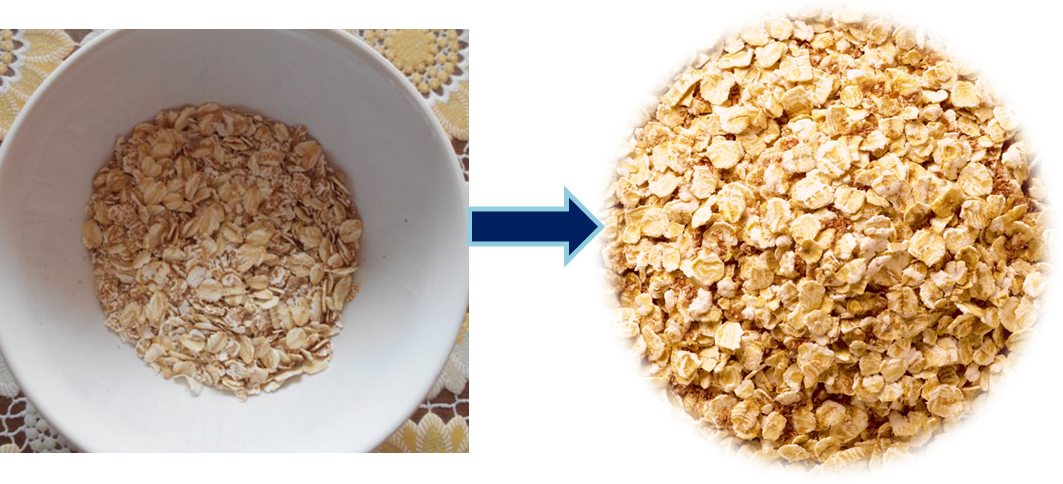
\includegraphics[width=0.8\textwidth]{media/pish2/image3}
	\caption*{}
\end{figure}


{\bfseries 2 - сурет. Жералмұртпен байытылған бидай кебегі мен сұлы жармасы
негізіндегі таңғы астың зертханалық нұсқасы}

Жералмұртпен байытылған бидай кебегі мен сұлы жармасына негізделген
құрғақ таңғы ас функционалды тамақтану үшін негізгі таңдау болады. Сұлы
жармасы-ақуыздың, витаминдердің және темір, мырыш және магний сияқты
минералдардың бай көзі. Оның құрамында ас қорытуды жақсартуға
көмектесетін талшық бар. Бидай кебегі-құрамында талшықтың көп мөлшері
бар, ол қанықтыруға және ішектің жұмысын жақсартуға көмектеседі.
Жералмұрт - инулиннің көзі, ол пребиотик болып табылады және ішек
микрофлорасына пайдалы әсер етеді. Жералмұрт құрамында калий мен магний
сияқты дәрумендер мен минералдар бар.

{\bfseries Қорытынды.} Осылайша, жералмұртпен байытылған бидай кебегі бар
сұлы жармасына негізделген таңғы асты әзірлеу пайдалы және қоректік
өнімді құрудың перспективалы бағыты болып табылады. Ингредиенттердің
ерекше құрамына байланысты бұл таңғы ас құрамында дәрумендер, минералдар
мен диеталық талшықтар көп болады, бұл жалпы денсаулықты жақсартуға және
күні бойы энергияны арттыруға көмектеседі. Мұндай өнімдерді әзірлеу
рационның әртүрлілігіне және функционалды тамақстануды қамтамасыз етеді.
Бұл технологияның, атап айтқанда, теңдестірілген құрамдағы немесе арнайы
мақсаттағы өнімдерді өндіру үшін үлкен перспективалары бар.

\emph{{\bfseries Қаржыландыру:} Жұмыс Қазақстан Республикасының Ауыл
шаруашылығы министрлігі BR 22886613 "Ауыл шаруашылығы Өсімдік
шаруашылығы өнімдері мен шикізатын қайта өңдеу және сақтау жөніндегі
инновациялық технологияларды әзірлеу" қаржыландыратын бағдарлама
шеңберінде жүргізілді.}

\emph{Қорытындылай келе, біз осы ғылыми жобаның барлық қатысушыларына
эксперименттік зерттеулер жүргізуге көмектескені үшін шын жүректен алғыс
айтқымыз келеді. Біз сондай-ақ "ҚазҒЗИ қайта өңдеу және тамақ
өнеркәсібі" ЖШС Астана филиалының басшылығы мен ғалымдарына алғысымызды
білдіреміз.}

Әдебиеттер

\begin{enumerate}
\def\labelenumi{\arabic{enumi}.}
\item
  Di Cairano M. et al. Functional cereal-based bakery products,
  breakfast cereals, and pasta products //Functional Cereals and Cereal
  Foods.- 2022. -P. 215-249. DOI 10.1007/978-3-031-05611-6\_9
\item
  Pаucean A., Man S., Pop A. Development of oat based-food formulation
  and quality characteristics // Journal of Agroalimentary Processes and
  Technologies. -2015.-Vol. 21(3). -P. 261-266.
\item
  Fulgoni III V. L. et al. Oatmeal-containing breakfast is associated
  with better diet quality and higher intake of key food groups and
  nutrients compared to other breakfasts in children //Nutrients. -
  2019. -Vol 11(5):964. DOI 10.3390/nu11050964
\item
  Rebello C.J. et al. Acute effect of oatmeal on subjective measures of
  appetite and satiety compared to a ready-to-eat breakfast cereal: a
  randomized crossover trial //Journal of the American college of
  nutrition. -2013. -Vol. 32(4). -P. 272-279.
  \href{https://doi.org/10.1080/07315724.2013.816614}{DOI
  10.1080/07315724.2013.816614}
\item
  Saini P. et al. Wheat bran as potential source of dietary fiber:
  Prospects and challenges //Journal of Food Composition and Analysis.
  -2023. -Vol. 116. DOI 10.1016/j.jfca.2022.105030
\item
  Hassanzadeh-Rostami Z., Abbasi A., Faghih S. Effects of biscuit
  fortified with whey protein isolate and wheat bran on weight loss,
  energy intake, appetite score, and appetite regulating hormones among
  overweight or obese adults //Journal of Functional Foods. -- 2020. -
  Vol. 70. DOI 10.1016/j.jff.2019.103743
\item
  Ганиева А.Ф. Исследование возможности использования ягодного сырья для
  повышения пищевой ценности хлебобулочных изделий / А.Ф. Ганиева, И.Т.
  Гареева, Д.Т. Гайфуллина // Состояние и перспективы увеличения
  производства высококачественной продукции сельского хозяйства.
  материалы VIII Международной научно-практической конференции, 2020. -
  С. 127-131.
\item
  Munim A. et al. An analysis of the composition, health benefits, and
  future market potential of the Jerusalem artichoke in Canada. -2017.
  -Vol. 6(5). -P. 69-84. DOI 10.5539/jfr.v6n5p69
\item
  Choton S. et al. Extrusion technology and its application in food
  processing: A review //The Pharma Innovation Journal. -2020. - Vol.
  9(2). - P. 162-168. DOI 10.22271/tpi.2020.v9.i2d.4367
\item
  Robin F., Palzer S. Texture of breakfast cereals and extruded products
  //Modifying food texture. -- Woodhead Publishing, 2015. -- P. 203-235.
  DOI 10.1016/B978-1-78242-333-1.00010-3
\end{enumerate}

{\bfseries References}

1.Di Cairano M. et al. Functional cereal-based bakery products,
breakfast cereals, and pasta products //Functional Cereals and Cereal
Foods.- 2022. -P. 215-249. DOI 10.1007/978-3-031-05611-6\_9

2.Pаucean A., Man S., Pop A. Development of oat based-food formulation
and quality characteristics // Journal of Agroalimentary Processes and
Technologies. -2015.-Vol. 21(3). -P. 261-266.

3.Fulgoni III V. L. et al. Oatmeal-containing breakfast is associated
with better diet quality and higher intake of key food groups and
nutrients compared to other breakfasts in children //Nutrients. - 2019.
-Vol 11(5):964. DOI 10.3390/nu11050964

4.Rebello C.J. et al. Acute effect of oatmeal on subjective measures of
appetite and satiety compared to a ready-to-eat breakfast cereal: a
randomized crossover trial //Journal of the American college of
nutrition. -2013. -Vol. 32(4). -P. 272-279.
\href{https://doi.org/10.1080/07315724.2013.816614}{DOI
10.1080/07315724.2013.816614}

5.Saini P. et al. Wheat bran as potential source of dietary fiber:
Prospects and challenges //Journal of Food Composition and Analysis.
-2023. -Vol. 116. DOI 10.1016/j.jfca.2022.105030

6.Hassanzadeh-Rostami Z., Abbasi A., Faghih S. Effects of biscuit
fortified with whey protein isolate and wheat bran on weight loss,
energy intake, appetite score, and appetite regulating hormones among
overweight or obese adults //Journal of Functional Foods. -- 2020. -
Vol. 70. DOI 10.1016/j.jff.2019.103743

7. Ganieva A.F. Issledovanie vozmozhnosti ispol' zovanija
jagodnogo syr' ja dlja povyshenija pishhevoj cennosti
hlebobulochnyh izdelij / A.F. Ganieva, I.T. Gareeva, D.T. Gajfullina //
Sostojanie i perspektivy uvelichenija proizvodstva vysokokachestvennoj
produkcii sel' skogo hozjajstva. materialy VIII
Mezhdunarodnoj nauchno-prakticheskoj konferencii, 2020. - S.
127-131.{[}in Russian{]}

8.Munim A. et al. An analysis of the composition, health benefits, and
future market potential of the Jerusalem artichoke in Canada. -2017.
-Vol. 6(5). -P. 69-84. DOI 10.5539/jfr.v6n5p69

9.Choton S. et al. Extrusion technology and its application in food
processing: A review //The Pharma Innovation Journal. -2020. - Vol.
9(2). - P. 162-168. DOI 10.22271/tpi.2020.v9.i2d.4367

10.Robin F., Palzer S. Texture of breakfast cereals and extruded
products //Modifying food texture. - Woodhead Publishing, 2015. - P.
203-235. DOI 10.1016/B978-1-78242-333-1.00010-3

\emph{{\bfseries Авторлар туралы мәліметтер}}

Султанова М.- техника ғылымдарының магистрі, «Қазақ қайта өңдеу және
тағам өнеркәсіптері ғылыми-зерттеу институты» ЖШС Астана филиалының жоба
жетекшісі, Астана, Қазақстан, e-mail: sultanova.2012@mail.ru;

Акжанов Н.- жаратылыстану ғылымдары магистрі, «Қазақ қайта өңдеу және
тағам өнеркәсіптері ғылыми-зерттеу институты» ЖШС Астана филиалының аға
ғылыми қызметкері, Астана,Қазақстан, e-mail: nurtore0308@gmail.com;

Садуакас А/- «Қазақ қайта өңдеу және тағам өнеркәсіптері ғылыми-зерттеу
институты» ЖШС Астана филиалының өсімдік шикізатын бастапқы өңдеу
зертханасының ғылыми қызметкері, Астана, Қазақстан, e-mail:
aykon96@mail.ru;

Камали А.- «Қазақ қайта өңдеу және тағам өнеркәсіптері ғылыми-зерттеу
институты» ЖШС Астана филиалының өсімдік шикізатын бастапқы өңдеу
зертханасының кіші ғылыми қызметкері, Астана,Қазақстан, e-mail:
akerke.kamali@bk.ru.

\emph{{\bfseries Information about the authors}}

Sultanova M.-Master of Technical Sciences, Project Manager of the Astana
Branch of the Kazakh Research Institute of Processing and Food
Industries LLP, Astana, Kazakhstan, e-mail: sultanova.2012@mail.ru;

Akzhanov N.- Master of Natural Sciences, Senior Researcher of the Astana
Branch of the Kazakh Research Institute of Processing and Food
Industries LLP, Astana, Kazakhstan, e-mail: nurtore0308@gmail.com;

Saduakas A.-Researcher of the Laboratory of Primary Processing of Plant
Raw Materials, Astana Branch of the Kazakh Research Institute of
Processing and Food Industries, Astana, Kazakhstan, e-mail:
aykon96@mail.ru;

Kamali A.- Junior Researcher of the Laboratory of Primary Processing of
Plant Raw Materials, Astana Branch of the Kazakh Research Institute of
Processing and Food Industries, Astana, Kazakhstan, e-mail:
akerke.kamali@bk.ru.